\chapter{Technology Details}

The technology details on the identifier renaming project has been published in paper ``A Neural Architecture for Detecting Identifier Renaming from Diff'' seen in \autoref{sec:produced-publications}.
This chapter hence presents technology details for the RM2HyperLedger project. I first explain the technology of RM2PT, then transition to RM2HyperLedger.

\section{RM2PT}

The RM2PT program written by Yang is an Eclipse plugin, written in Xtend, a Java dialect. The main input to RM2PT is a \code{.remodel} file, which is a requirement document written in Yang's  domain specific language. \autoref{yang-dls} is an abridged \code{.remodel} file. The exact language specification is unknown, but the contract definition part is in Object Constraint Language (OCL).

\begin{figure}[ht]
\begin{lstlisting}[language={}, breaklines=true, showstringspaces=false, frame=tb, caption={an abridged \code{.remodel} file. The contract definition part is written in OCL.}, label=yang-dls]
UseCaseModel CoCoME {
	UC::processSale() definedBySSD(ProcessSaleSSD) relatedService(ProcessSaleService)
	UC::openCashDesk()

	Actor Cashier {
		processSale
		openCashDesk
		closeCashDesk
	}

	Contract  ManageSupplierCRUDService::deleteSupplier(id : Integer) : Boolean {

		/* definition: find specific Supplier instance by id */
		definition:
			supplier:Supplier = Supplier.allInstance()->any(sup:Supplier | sup.Id = id)

		/* precondition: the instance supplier was found in the system */
		precondition:
			supplier.oclIsUndefined() = false and
			Supplier.allInstance()->includes(supplier)

		/* postcondition: the instance supplier was deleted from the system */
		postcondition:
			Supplier.allInstance()->excludes(supplier) and
			result = true
	}
}

DomainModel CoCoME {
	@AutoCRUD
	Entity ProductCatalog {
		Id : Integer
		Name : String

		[Refer]
		ContainedItems : Item* Association
		[INV]
		inv UniqueProductCatalogId : ProductCatalog.allInstance()->isUnique(p:ProductCatalog | p.Id)
	}
}
\end{lstlisting}
\end{figure}

\begin{figure}[ht]
\centering
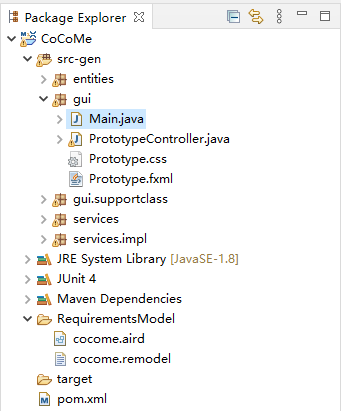
\includegraphics[width=0.5\linewidth]{rm2pt-folder-structure}
\caption{The project structure of a RM2PT project where all Java source code is auto-generated, grouped in the \code{src-gen} folder.}
\label{fig:rm2pt-folder-structure}
\end{figure}

\begin{figure}
\centering
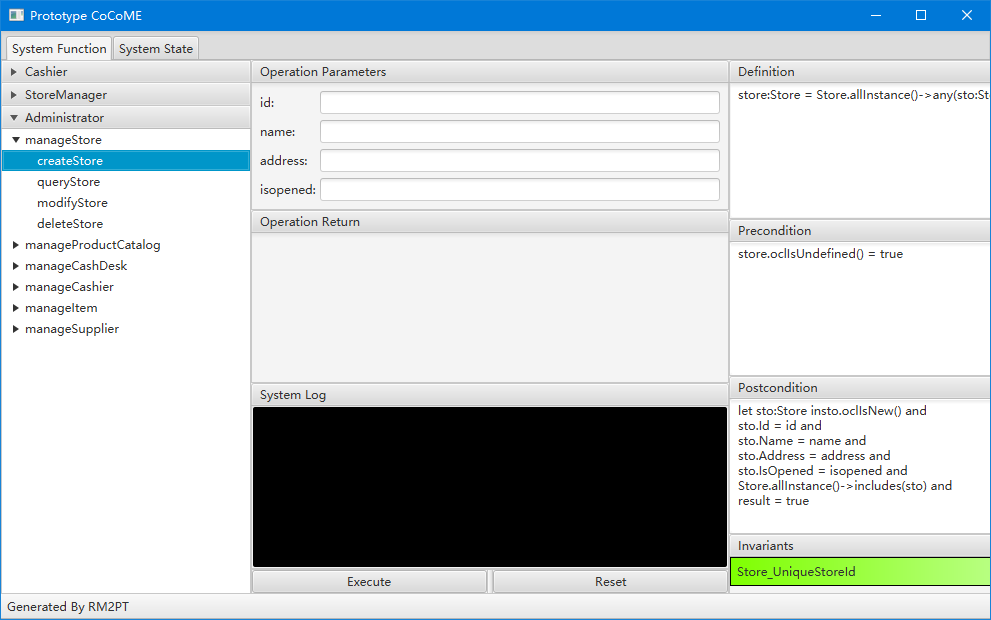
\includegraphics[width=0.7\linewidth]{cocome-javafx}
\caption{Screenshot of the desktop application generated by RM2PT}
\label{fig:cocome-javafx}
\end{figure}


RM2PT thus translates a \code{.remodel} file to a JavaFX project. The project structure is shown in~\autoref{fig:rm2pt-folder-structure} and all Java source code is auto-generated, grouped in the \code{src-gen} folder.
The project is a desktop application with a GUI implemented in JavaFX. \autoref{fig:cocome-javafx}~is a screenshot of the JavaFX prototype.


\section{RM2HyperLedger}

I am currently developing RM2HyperLedger, a program that translates requirements to HyperLedger chaincode.

Unlike RM2PT, RM2HyperLedger is a standalone application written in Java, not relying on Eclipse as many developers use IntelliJ Idea or other IDEs. For now RM2HyperLedger takes as input the \code{.remodel} file and the generated JavaFX code. RM2HyperLedger uses Antlr to analyze Java source code and translate to the HyperLedger Fabric format.

I have encoded the following translation rules in RM2HyperLedger.

\begin{itemize}
\item Add or locate system level identifier (PK) of each entity.
\item Add serialization support to each entity.
\item Store serialized objects to blockchain, and retrieve them by their PK.
\item Rewrite method signatures to fit HyperLedger Fabric format.
\item When a new object is created or an object is deleted from memory, synchronize with the blockchain.
%\item etc.
\end{itemize}

I am still going to formalize and encode more rules, for example
1) when an object is modified, synchronize with the blockchain;
2) rewrite class definition to fit HyperLedger Fabric format;
3) automatically generate test code;
and so on.
